% !TEX encoding = UTF-8 Unicode
% !TEX TS-program = pdflatex
% !TEX spellcheck = it-IT

\section{Visione generale della strategia}
	\subsection{Procedure di controllo di qualità di processo}
		Per garantire la qualità dei processi e quindi un loro miglioramento continuo verrà usato il principio \gl{PDCA}. Di conseguenza migliorerà la qualità del \gl{prodotto}. \\
		Per avere il controllo dei processi, e di conseguenza qualità, è necessario che:
		\begin{itemize}
			\item\ i processi siano pianificati dettagliatamente;
			\item\ vi sia un controllo sul lavoro di ogni membro del \gl{team};
			\item\ nella pianificazione siano ripartite chiaramente le risorse.
		\end{itemize}
		L'attuazione di questi punti è approfondita nel \PPdoc. \\
		Analizzando la qualità del \gl{prodotto} si controlla anche la qualità dei processi. Un \gl{prodotto} scadente indica che i processi sono migliorabili. \\
		Inoltre si possono usare delle metriche per quantificare la qualità dei processi, tali metriche sono descritte nella sezione \hyperref[sec:3.9]{3.9 Misure e metriche}.
	\subsection{Procedure di controllo di qualità di \gl{prodotto}}
		Il controllo di qualità del \gl{prodotto} verrà garantito da:
		\begin{itemize}
			\item \textbf{quality assurance:} è l'insieme di attività realizzate per raggiungere gli obiettivi di qualità. Queste attività prevedono l'attuazione di tecniche di analisi statica e dinamica, descritte nella sezione \hyperref[sec:3.8]{3.8 Tecniche di analisi}.
			\item \textbf{verifica:} è un processo che determina se l'output di una fase è consistente, corretto e completo. Per tutta la durata del \gl{progetto} verranno svolte attività di verifica, i cui risultati sono e saranno riportati nell'\hyperref[sec:A]{Appendice A}.
			\item \textbf{validazione:} è il processo di conferma oggettiva del soddisfacimento dei requisiti, attuato per ogni fase del \gl{progetto}.
		\end{itemize}
	\subsection{Organizzazione}
		L'organizzazione della strategia di verifica si basa sull'attuazione di verifiche per ogni processo completato. Queste verifiche controllano sia la qualità del processo stesso sia la qualità del \gl{prodotto} ottenuto. Grazie al diario delle modifiche sarà possibile eseguire una verifica solo sui cambiamenti effettuati. \\
		A causa della diversa natura dei risultati ottenuti da ogni fase del processo ognuno di essi richiederà l'attuazione di specifiche procedure di verifica. Il \gl{team} ha deciso di adottare un ciclo di vita \gl{incrementale} per lo sviluppo del \gl{progetto}. Di conseguenza il processo di verifica adottato per ogni fase del \gl{progetto} opererà nel modo seguente:
		\begin{itemize}
			\item \textbf{A e B:} in questa fase verranno redatti i documenti che riporteranno i requisiti individuati, le strategie e le norme adottate.
			\begin{itemize}
				\item Verrà controllata la correttezza ortografica con il correttore automatico di \gl{TeXstudio}.
				\item Verrà controllata la correttezza lessicale con un'attenta ed accurata rilettura.
				\item Verrà controllata la correttezza dei contenuti rispetto alle aspettative del documento attraverso una rilettura accurata.
				\item Verrà verificato che ogni requisito abbia una corrispondenza in un caso d'uso; per farlo si controlleranno le apposite tabelle di tracciamento, con l'ausilio di \gl{Trender}.
				\item Ogni documento dovrà rispettare le \NPdoc; per verificarlo verranno adoperati gli strumenti più appropriati.
				\item Verrà verificato che sia presente una didascalia per ogni rappresentazione grafica e il contenuto di ogni figura e tabella.
			\end{itemize}
			\item \textbf{C:} verrà garantito che ogni requisito possa essere rintracciabile, attraverso il processo di verifica. Ogni requisito sarà rintracciabile nei componenti individuati in questa fase, si veda la \hyperref[sec:2]{Sezione 2}\ per ulteriori approfondimenti.
			\item \textbf{D, E e F:} i Programmatori svolgeranno le attività di codifica e di esecuzione dei test di unità per la verifica del codice. Queste attività avverranno nel modo più automatizzato possibile, rispettando anche i vincoli statici. I Verificatori controlleranno parallelamente la presenza di eventuali anomalie, definite nella \hyperref[sec:4]{Sezione 4}.
			\item \textbf{G:} alla Revisione di Accettazione (RA) il gruppo \AUTORE\ garantisce il funzionamento corretto del \gl{prodotto} realizzato. Le eventuali modifiche per eliminare le possibili diversità rispetto al \gl{prodotto} atteso saranno a carico del \gl{proponente}.
		\end{itemize}
		In ogni documento viene inoltre incluso il diario delle modifiche, in modo da mantenere uno storico delle attività svolte e delle relative responsabilità.
	\subsection{Pianificazione strategica e temporale}
		Per impedire una rapida diffusione degli errori è necessario che la verifica della documentazione sia sistematica ed organizzata. In questo modo inoltre l'individuazione e la correzione degli errori avverrà il prima possibile. \\
		Nel \PPdoc verranno pianificate le attività svolte per migliorare la qualità dei processi, le quali stabiliranno delle nuove norme di \gl{progetto}. \\
		Per ridurre la possibilità di commettere errori e/o imprecisioni di natura tecnica/concettuale ogni attività di redazione o di codifica dovrà essere preceduta da uno studio preliminare. In questo modo viene alleggerita l'attività di verifica perché richiederà a posteriori meno interventi correttivi. \\
		Il \gl{team} ha come obiettivo il rispetto delle scadenze fissate nel \PPdoc, riportate di seguito:
		\begin{itemize}
			\item\ revisioni formali:
			\begin{itemize}
				\item\ Revisione dei Requisiti: 2016/04/18.
				\item\ Revisione di Accettazione: 2016/09/12.
			\end{itemize}
			\item revisioni di progresso:
			\begin{itemize}
				\item\ Revisione di Progettazione: 2016/06/17.
				\item\ Revisione di Qualifica: 2016/08/24.
			\end{itemize}
		\end{itemize}
	\subsection{Responsabilità}
		La responsabilità dell'assegnazione degli incarichi è a carico del \RES. L'\AM\ avrà come responsabilità l'adeguamento dell'ambiente di lavoro per lo svolgimento di tutti i compiti necessari alla realizzazione del \gl{progetto}. Ogni componente del \gl{team} è responsabile del proprio materiale \gl{prodotto}.
	\subsection{Risorse}
		\subsubsection{Necessarie}
			Per la realizzazione del \gl{prodotto} sono necessarie risorse sia tecnologiche che umane:
			\begin{itemize}
				\item \textbf{risorse umane:}\ vengono descritte dettagliatamente nel \PPdoc.
				\begin{itemize}
					\item\ Amministratore;
					\item\ Responsabile;
					\item\ Analista;
					\item\ Progettista;
					\item\ Programmatore;
					\item\ Verificatore.
				\end{itemize}
				\item \textbf{risorse \gl{software}:} sono necessari strumenti \gl{software} utili:
				\begin{itemize}
					\item\ alla stesura di documentazione in \gl{LaTeX};
					\item\ alla creazione di diagrammi in \gl{UML};
					\item\ allo sviluppo nei linguaggi di programmazione scelti;
					\item\ a semplificare ed automatizzare la verifica;
					\item\ all'analisi statica del codice;
					\item\ alla gestione dei test sul codice.
				\end{itemize}
				\item \textbf{risorse \gl{hardware}:} sono necessari computer con tutti gli strumenti \gl{software} descritti nelle \NPdoc. È necessario avere a disposizione uno o più luoghi dove poter effettuare le riunioni interne del gruppo \AUTORE. Sono necessari i \gl{beacon} in un numero sufficiente per i test del \gl{progetto}. È necessario avere un server su cui installare il database necessario per il funzionamento del \gl{prodotto}. Sono necessari degli \gl{smartphone} adatti ad eseguire i test del \gl{prodotto}.
			\end{itemize}
		\subsubsection{Disponibili}
			Ogni membro di \AUTORE\ ha a disposizione almeno un computer personale dotato di tutti gli strumenti necessari con cui poter svolgere tutti i propri compiti. \\
			A scopo di test, di supporto degli strumenti scelti per l'ambiente di sviluppo, e per il funzionamento dell'app vengono messi a disposizione uno spazio web e un server privato da \PROPONENTE. \\
			Per lo svolgimento delle riunioni interne il \gl{team} usa le aule del Dipartimento di Matematica dell'Università degli Studi di Padova; inoltre usa \gl{Google Hangouts} come strumento di discussione tramite videochiamate.
	\subsection{Strumenti}
		Nella sezione ‘‘Ambiente di sviluppo’’ del documento \NPdoc sono descritti gli strumenti \gl{software} impiegati dal \gl{team} per:
		\begin{itemize}
			\item\ il versionamento;
			\item\ la redazione e la verifica di documenti;
			\item\ la stesura e la verifica del codice;
			\item\ la semplificazione del lavoro tramite la stesura di \gl{script}; %visto che la Vivi ha fatto lo \gl{script} per trovare le parole con \gl penso si possa lasciare quest'affermazione
			\item\ l'organizzazione e la condivisione dei file.
		\end{itemize}
	\subsection{Tecniche di analisi}
		\label{sec:3.8}
		\subsubsection{Analisi statica}
			L'analisi statica è una tecnica di verifica applicabile sia ai documenti che al codice. Verrà effettuata per tutta la fase di sviluppo del \gl{progetto} e serve per trovare anomalie, che verranno trattate come descritto nelle \NPdoc. Può essere applicata nei due modi seguenti.
			\paragraph{Walkthrough}
				Consiste in una lettura del documento/codice cercando anomalie ed errori ad ampio spettro, cioè senza avere un'idea precisa di quali possibili errori si potranno trovare. Per evitare incomprensioni ogni modifica verrà discussa con gli autori e concordata tra le due parti. \\
				Il \gl{walkthrough}\ è una tecnica indispensabile nelle prime fasi di sviluppo, in cui non si ha un'idea precisa dei possibili errori. Usando questa tecnica sarà poi possibile stilare una ‘‘lista di controllo’’, dove verranno archiviati gli errori più frequenti. Tale lista sarà salvata nell'Appendice delle \NPdoc. \\ %quest'ultima frase sarà da decidere se tenere o no e quindi agire di conseguenza
				Inizialmente le fasi di verifica prevederanno perlopiù l'uso della tecnica \gl{walkthrough}. Appena la lista di controllo sarà sufficientemente ampia si userà sempre di più la tecnica di \gl{Inspection}.
			\paragraph{Inspection}
				L'\gl{inspection}\ si basa sulla lettura mirata dei documenti/codice, cercando gli errori segnalati nella lista di controllo. Man mano che le verifiche procedono la lista verrà estesa e l'\gl{inspection}\ sarà più efficace.
		\subsubsection{Analisi dinamica}
			L'analisi dinamica verifica il funzionamento delle sole componenti \gl{software} tramite dei test e aiuta ad identificarne le anomalie. \\
			Per garantire un risultato attendibile il test dev'essere ripetibile, ovvero deve ottenere sempre lo stesso output dallo stesso input quando viene eseguito nello stesso ambiente. Solo così il test garantisce di trovare eventuali problemi e quindi verificare la correttezza del \gl{prodotto} \gl{software}. \\
			Per ogni test dev'essere definito:
			\begin{itemize}
				\item \textbf{ambiente:} è l'insieme dei sistemi \gl{hardware} e \gl{software} sui quali viene pianificata l'esecuzione del test sul \gl{prodotto}. Va inoltre specificato uno stato iniziale da cui il test deve partire;
				\item \textbf{specifica:} consiste nella specifica degli input e degli output attesi;
				\item \textbf{procedure:} è la specifica di ulteriori istruzioni sull'esecuzione del test e sull'interpretazione dei risultati.
			\end{itemize}
			Nelle prossime sezioni sono definiti i tipi di test effettuati sul \gl{prodotto} \gl{software} in sviluppo dal \gl{team}.
			\paragraph{Test di unità}
				Il test di unità verifica che ogni singola unità di \gl{prodotto} funzioni correttamente. Per unità si intende una porzione di \gl{software} abbastanza piccola da poterne assegnare lo sviluppo ad un singolo \PR. \\
				Attraverso questo test verrà verificata la correttezza di ogni modulo base che compone il \gl{software}, limitando gli errori di implementazione. \\
				I test di unità sono identificati dalla seguente sintassi:
				\begin{center}
					TU[Codice test]
				\end{center}
			\paragraph{Test di integrazione}
				Il test di integrazione verifica che due o più moduli già verificati funzionino come previsto quando vengono assemblati insieme. Inoltre aiuta a scovare i difetti residui sfuggiti dalla fase di test precedente. \\
				In più con questo test viene verificata la collaborazione tra i moduli prodotti e le componenti esterne usate come \gl{framework} o librerie. \\
				È possibile che vengano usate delle componenti ‘‘fittizie’’ al posto dei moduli non ancora completati per poter eseguire comunque dei test. \\
				I test di integrazione sono identificati dalla seguente sintassi:
				\begin{center}
					TI[identificativo del componente]
				\end{center}
				Tale identificativo corrisponde al componente i cui elementi sono integrati.
			\paragraph{Test di sistema}
				I test di sistema validano l'intero \gl{prodotto} \gl{software} quando si ritiene che esso sia giunto ad una versione definitiva. Viene quindi controllato se tutti i requisiti sono stati soddisfatti. \\
				I test di sistema sono identificati dalla seguente sintassi:
				\begin{center}
					TS[Tipo Requisito][Codice Requisito]
				\end{center}
				Il tipo e il codice si riferiscono al requisito di cui verrà testato il soddisfacimento.
			\paragraph{Test di regressione}
				Questo test viene eseguito dopo la modifica di una componente, e consiste nel rieseguire tutti i test. In questo modo si controlla che dopo la modifica tutti i moduli continuino a funzionare correttamente. \\
				Il tracciamento aiuta a capire quali sono i test da ripetere (di ogni tipo) poiché potenzialmente a rischio in caso di modifica.
			\paragraph{Test di validazione}
				Coincide con il collaudo del \gl{software} in presenza del \gl{proponente}. Se il test risulta positivo il \gl{prodotto} sarà considerato sufficientemente maturo da permetterne il rilascio. \\
				I test di validazione sono identificati dalla seguente sintassi:
				\begin{center}
					TV[Tipo Requisito][Codice Requisito]
				\end{center}
				Il tipo e il codice si riferiscono al requisito di cui verrà testato il soddisfacimento.
			\paragraph{Modello a V}
				Per la pianificazione dei test si utilizzerà il Modello a V. Secondo questo modello il testing del software viene suddiviso in livelli differenti, i quali si concretizzano in un'esecuzione bottom-up che avanza sequenzialmente alle attività di codifica e di validazione. Ad ogni livello corrisponde un ciclo di uno specifico tipo di test, ed ogni test viene creato in base al relativo livello di progettazione.
				\begin{figure}
					\centering
					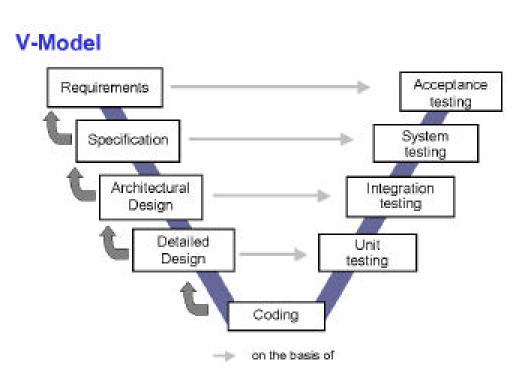
\includegraphics[width=0.5\textwidth]{img/V-model.jpg}
					\caption{Modello a V}
				\end{figure}
			\paragraph{Tracciamento}
				Sarà compito dei Verificatori controllare la corrispondenza di ogni requisito con una o più fonti. In caso di anomalie bisogna comportarsi come descritto [NOTA PER IL VERIFICATORE: bisogna controllare se da qualche parte c'è una procedura per informare della presenza dell'anomalia e scrivere quindi qui il riferimento].
	\subsection{Misure e metriche}
		\label{sec:3.9}
		Per essere utile ed informativo il processo di verifica dev'essere quantificabile. Vanno quindi stabilite a priori delle metriche, sulle quali saranno basate le misure rilevate dal processo di verifica. Nel caso in cui vi fossero delle metriche approssimate ed incerte, esse miglioreranno in modo \gl{incrementale}. Questo grazie al ciclo di vita adottato descritto nel \PPdoc. Possono esserci due tipi di \gl{range}:
		\begin{itemize}
			\item \textbf{\gl{range} di accettazione:}\ insieme di valori richiesti affinché il \gl{prodotto} sia accettato.
			\item \textbf{\gl{range} ottimale:}\ insieme di valori entro i quali dovrebbe collocarsi la misurazione. Esso non è vincolante, ma fortemente consigliato. Scostamenti da tali valori necessitano una verifica approfondita.
		\end{itemize}
		\subsubsection{Metriche per i processi}
			\label{sec:3.9.1}
			\paragraph{Valutazione \gl{CMM}}
				\label{sec:3.9.1.1}
				I processi verranno valutati secondo il modello \gl{CMM}. Tale modello prevede che ogni processo verrà valutato secondo le proprie ‘‘Capability’’ e ‘‘Maturity’’. Per entrambe verrà assegnato un voto da 1 (stato iniziale) a 5 (stato controllato), che ne indicherà la valutazione complessiva. \\
				La scelta di \gl{CMM} rispetto ai più recenti CMMI e \iso{\gl{ISO}/IEC 15504} è dovuta alla maggior snellezza della valutazione. Il primo valuta usando solo due parametri, i secondi invece dividono il processo in più attributi. \\
				È stata fatta questa scelta a causa del \gl{progetto} non molto grande. Questo renderebbe alcuni attributi superflui o sopravvalutati. Altri due elementi che hanno portato a questa scelta sono l'inesperienza del gruppo e la rotazione dei ruoli. Questi porterebbero a facili fraintendimenti e disaccordi sulle singole valutazioni.
				
				\textbf{Parametri utilizzati:}
				\begin{itemize}
					\item \textbf{Range accettazione:}\ 3 - 5;
					\item \textbf{Range ottimale:}\ 4 - 5.
				\end{itemize}
		\subsubsection{Metriche per i documenti}
			\label{sec:3.9.2}
			\paragraph{Indice \gl{Gulpease}}
				\label{sec:3.9.2.1}
				L'indice \gl{Gulpease} è un indice di leggibilità del testo creato appositamente per valutare la lingua italiana. Dato che non valuta la lunghezza delle parole mediante il numero di sillabe tale indice semplifica il calcolo rispetto ad altri indici di leggibilità. Esso infatti è basato sul numero di caratteri contenuti in una parola e ad altri fattori come il numero di parole e di frasi. Come tutti gli indici di leggibilità esso permette di indicare la complessità di un documento. Il calcolo da effettuare è il seguente:
				\[89+\frac{300(numero\,\, delle\,\, frasi) - 10(numero\,\, delle\,\, lettere)}{numero\,\, delle\,\, parole}\]
				I risultati sono compresi tra 0 e 100, dove 100 è il valore di leggibilità più alto e 0 quello più basso. Sono state stabilite delle soglie per rapportare il livello di istruzione di un individuo con i vari gradi dell'indice:
				\begin{itemize}
					\item \textbf{inferiore a 80:} documento difficile da leggere per chi ha la licenza elementare;
					\item \textbf{inferiore a 60:} documento difficile da leggere per chi ha licenza media;
					\item \textbf{inferiore a 40:} documento difficile da leggere per chi ha la licenza superiore.
				\end{itemize}
				In realtà tale indice non certifica se il testo sia comprensibile o meno. Per lo scopo dei documenti e per la formalità richiesti da essi verranno usati spesso termini tecnici che non si possono sostituire. Di conseguenza un documento potrebbe avere un ottimo indice di \gl{Gulpease} ma essere difficile da comprendere per i termini usati. Anche spezzare una frase può migliorare l'indice, ma interromperebbe il ragionamento fatto in quella frase. Infine usare frasi troppo dirette potrebbe essere poco professionale ai fini del documento. Per queste ragioni i documenti verranno valutati da un essere umano, così potrà stabilire se il testo è semplificabile. I limiti imposti da tale indice saranno sufficientemente rilassati per accettare frasi un po' più articolate.
				
				\textbf{Parametri utilizzati:}
				\begin{itemize}
					\item \textbf{Range accettazione:}\ 40- 100;
					\item \textbf{Range ottimale:}\ 50 - 100.
				\end{itemize}
		\subsubsection{Metriche per il codice}		
			\label{sec:3.9.3}
			\paragraph{Numero di parametri}
				\label{sec:3.9.3.1}
				Indica il numero di parametri formali in input di un metodo. Se il numero di parametri è elevato, lo \gl{stack} del programma può essere riempito rapidamente in caso di chiamate multiple innestate. I costruttori potranno superare questo limite se il numero elevato di parametri potrà facilitare la verifica tramite test e rendere più robusto agli errori l'oggetto definito.
				
				\textbf{Parametri utilizzati:}
				\begin{itemize}
					\item \textbf{Range accettazione:}\ 0 - 8;
					\item \textbf{Range ottimale:}\ 0 - 5.
				\end{itemize}
			\paragraph{Complessità ciclomatica}
				\label{sec:3.9.3.2}
				Indica il numero di cammini linearmente indipendenti che attraversano il grafo di flusso di controllo del metodo. In tale grafo i nodi rappresentano unità atomiche di istruzioni. Gli archi indicano che le istruzioni collegate dai nodi collegati possono essere eseguite consecutivamente. \\
				Un alto valore di complessità si può ridurre con la suddivisione in più metodi. È accettata anche una misurazione più lasca se questo dovesse influire in modo positivo sulla velocità di esecuzione. Oltretutto un valore alto potrebbe essere causato da strutture che in realtà aiutano ad ordinare il codice, come gli switch di condizioni.
				
				\textbf{Parametri utilizzati:}
				\begin{itemize}
					\item \textbf{Range accettazione:}\ 0 - 10;
					\item \textbf{Range ottimale:}\ 0 - 6.
				\end{itemize}
			\paragraph{Numero di campi dati per classe}
				\label{sec:3.9.3.3}
				Un elevato numero di attributi interni rende la classe troppo poco specializzata, ed è indice di cattiva progettazione. Dato che la classe ricoprirà più ruoli, rende anche più difficile il mantenimento del codice. \\
				La riduzione del numero dei campi dati si può ottenere con l'incapsulamento in nuove classi.
				
				\textbf{Parametri utilizzati:}
				\begin{itemize}
					\item \textbf{Range accettazione:}\ 0 - 16;
					\item \textbf{Range ottimale:}\ 0 - 10.
				\end{itemize}
			\paragraph{Livello d'annidamento}
				\label{sec:3.9.3.4}
				Indica quante volte le strutture di controllo sono state inserite l'una all'interno dell'altra. Un alto valore può portare a difficoltà nella verifica e nell'astrazione del codice.
				
				\textbf{Parametri utilizzati:}
				\begin{itemize}
					\item \textbf{Range accettazione:}\ 0 - 6;
					\item \textbf{Range ottimale:}\ 0 -4.
				\end{itemize}
			\paragraph{Grado di accoppiamento}
				\label{sec:3.9.3.5}
				È derivato da due singoli indici.
				\begin{itemize}
					\item \textbf{Indice di utilità:}\ numero di classi esterne al package che dipendono da classi al suo interno. Se il numero è basso il package non fornirà molte funzionalità e sarà poco utile. Se invece è alto troppe classi saranno dipendenti da tale package, rischiando di dover effettuare troppi cambiamenti ad ogni sua modifica.
					
					\textbf{Indice di utilità - Parametri utilizzati:}
					\begin{itemize}
						\item \textbf{Range accettazione:}\ 0 - 16;
						\item \textbf{Range ottimale:}\ 0 - 8.
					\end{itemize}
					\item \textbf{Indice di dipendenza:}\ numero di classi interne al package dipendenti da classi esterne. Un alto numero può indicare una scarsa progettazione.
					
					\textbf{Indice di dipendenza - Parametri utilizzati:}
					\begin{itemize}
						\item \textbf{Range accettazione:}\ 0 - 32;
						\item \textbf{Range ottimale:}\ 0 - 16.
					\end{itemize}
				\end{itemize}
			\paragraph{Chiamate innestate di metodi}
				\label{sec:3.9.3.6}
				Un grande numero di chiamate innestate di metodi può portare alla saturazione dello \gl{stack}, soprattutto in caso di un grande numero di parametri, quindi è necessario limitarne il numero.
				
				\textbf{Parametri utilizzati:}
				\begin{itemize}
					\item \textbf{Range accettazione:}\ 0 - 8;
					\item \textbf{Range ottimale:}\ 0 - 5.
				\end{itemize}
			\paragraph{Riepilogo}
				\begin{tabella}{!{\VRule}l!{\VRule}l!{\VRule}l!{\VRule}}
					\intestazionethreecol{Metriche}{Range accettazione}{Range ottimale}
					\hyperref[sec:3.9.1]{3.9.1 Metriche per i processi} & & \\
					\hyperref[sec:3.9.1.1]{3.9.1.1 Valutazione \gl{CMM}} & 3 -5 & 4 - 5 \\
					\hyperref[sec:3.9.2]{3.9.2 Metriche per i documenti} & & \\
					\hyperref[sec:3.9.2.1]{3.9.2.1 Indice \gl{Gulpease}} & 40 - 100 & 50 - 100 \\
					\hyperref[sec:3.9.3]{3.9.3 Metriche per il codice} & & \\
					\hyperref[sec:3.9.3.1]{3.9.3.1 Numero di parametri} & 0 - 8 & 0 - 5 \\
					\hyperref[sec:3.9.3.2]{3.9.3.2 Complessità ciclomatica} & 0 - 10 & 0 - 6 \\
					\hyperref[sec:3.9.3.3]{3.9.3.3 Numero campi dati per classe} & 0 -16 & 0 - 10 \\
					\hyperref[sec:3.9.3.4]{3.9.3.4 Livello d'annidamento} & 0 - 6 & 0 - 4 \\
					\hyperref[sec:3.9.3.5]{3.9.3.5 Grado di accoppiamento - Indice di utilità} & 0 - 16 & 0 - 8 \\
					\hyperref[sec:3.9.3.5]{3.9.3.5 Grado di accoppiamento - Indice di dipendenza} & 0 - 32 & 0 - 16 \\
					\hyperref[sec:3.9.3.6]{3.9.3.6 Chiamate innestate di metodi} & 0 - 8 & 0 - 5 \\
					
					\hiderowcolors
					\caption{Riepilogo delle metriche e dei \gl{range} di accettazione e ottimali}
				\end{tabella}